\documentclass{standalone}
\usepackage{tikz}
\usetikzlibrary{patterns, positioning}


\begin{document}
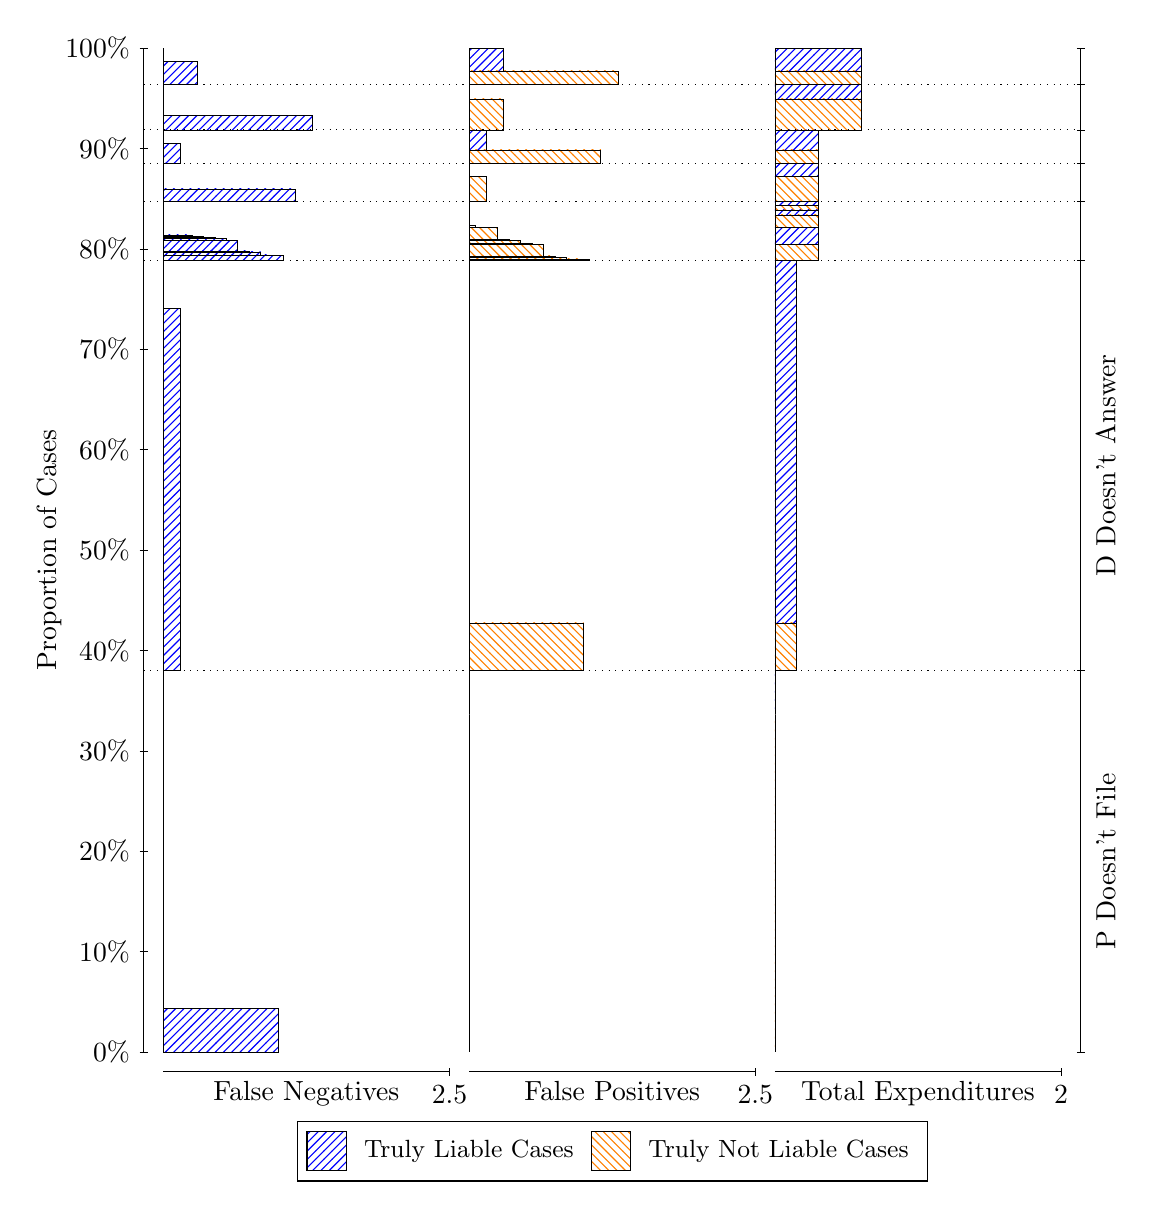
\begin{tikzpicture}
\draw[black, very thin] (1.5,1.75) -- (1.5,14.5);
\node[rotate=90, text=black, anchor=center] at (0.3, 8.125) {Proportion of Cases};
\draw[black, very thin] (1.45,1.75) -- (1.55,1.75);
\node[text=black, anchor=east] at (1.45, 1.75) {0\%};
\draw[black, very thin] (1.45,3.025) -- (1.55,3.025);
\node[text=black, anchor=east] at (1.45, 3.025) {10\%};
\draw[black, very thin] (1.45,4.3) -- (1.55,4.3);
\node[text=black, anchor=east] at (1.45, 4.3) {20\%};
\draw[black, very thin] (1.45,5.575) -- (1.55,5.575);
\node[text=black, anchor=east] at (1.45, 5.575) {30\%};
\draw[black, very thin] (1.45,6.85) -- (1.55,6.85);
\node[text=black, anchor=east] at (1.45, 6.85) {40\%};
\draw[black, very thin] (1.45,8.125) -- (1.55,8.125);
\node[text=black, anchor=east] at (1.45, 8.125) {50\%};
\draw[black, very thin] (1.45,9.4) -- (1.55,9.4);
\node[text=black, anchor=east] at (1.45, 9.4) {60\%};
\draw[black, very thin] (1.45,10.675) -- (1.55,10.675);
\node[text=black, anchor=east] at (1.45, 10.675) {70\%};
\draw[black, very thin] (1.45,11.95) -- (1.55,11.95);
\node[text=black, anchor=east] at (1.45, 11.95) {80\%};
\draw[black, very thin] (1.45,13.225) -- (1.55,13.225);
\node[text=black, anchor=east] at (1.45, 13.225) {90\%};
\draw[black, very thin] (1.45,14.5) -- (1.55,14.5);
\node[text=black, anchor=east] at (1.45, 14.5) {100\%};

\draw[black, very thin] (13.4,1.75) -- (13.4,14.5);
\draw[black, very thin] (13.35,1.75) -- (13.45,1.75);
\node[anchor=west] at (13.35, 1.75) {};
\draw[black, very thin] (13.35,6.5927) -- (13.45,6.5927);
\node[anchor=west] at (13.35, 6.5927) {};
\draw[black, very thin] (13.35,11.803) -- (13.45,11.803);
\node[anchor=west] at (13.35, 11.803) {};
\draw[black, very thin] (13.35,12.548) -- (13.45,12.548);
\node[anchor=west] at (13.35, 12.548) {};
\draw[black, very thin] (13.35,13.036) -- (13.45,13.036);
\node[anchor=west] at (13.35, 13.036) {};
\draw[black, very thin] (13.35,13.46) -- (13.45,13.46);
\node[anchor=west] at (13.35, 13.46) {};
\draw[black, very thin] (13.35,14.038) -- (13.45,14.038);
\node[anchor=west] at (13.35, 14.038) {};
\draw[black, very thin] (13.35,14.5) -- (13.45,14.5);
\node[anchor=west] at (13.35, 14.5) {};

\draw[black, very thin, pattern color=blue, pattern=north east lines] (1.75,1.75) rectangle (3.2033,2.3049);
\draw[black, very thin, pattern color=orange, pattern=north west lines] (1.75,2.3049) rectangle (1.75,6.5927);
\draw[black, very thin, pattern color=blue, pattern=north east lines] (1.75,6.5927) rectangle (1.968,11.195);
\draw[black, very thin, pattern color=orange, pattern=north west lines] (1.75,11.195) rectangle (1.75,11.803);
\draw[black, very thin, pattern color=blue, pattern=north east lines] (1.75,11.803) rectangle (3.276,11.867);
\draw[black, very thin, pattern color=blue, pattern=north east lines] (1.75,11.867) rectangle (3.1307,11.872);
\draw[black, very thin, pattern color=blue, pattern=north east lines] (1.75,11.872) rectangle (2.9853,11.911);
\draw[black, very thin, pattern color=blue, pattern=north east lines] (1.75,11.911) rectangle (2.84,11.923);
\draw[black, very thin, pattern color=blue, pattern=north east lines] (1.75,11.923) rectangle (2.6947,12.06);
\draw[black, very thin, pattern color=blue, pattern=north east lines] (1.75,12.06) rectangle (2.5493,12.079);
\draw[black, very thin, pattern color=blue, pattern=north east lines] (1.75,12.079) rectangle (2.404,12.099);
\draw[black, very thin, pattern color=blue, pattern=north east lines] (1.75,12.099) rectangle (2.2587,12.104);
\draw[black, very thin, pattern color=blue, pattern=north east lines] (1.75,12.104) rectangle (2.1133,12.126);
\draw[black, very thin, pattern color=orange, pattern=north west lines] (1.75,12.126) rectangle (1.75,12.548);
\draw[black, very thin, pattern color=blue, pattern=north east lines] (1.75,12.548) rectangle (3.4213,12.711);
\draw[black, very thin, pattern color=orange, pattern=north west lines] (1.75,12.711) rectangle (1.75,13.036);
\draw[black, very thin, pattern color=blue, pattern=north east lines] (1.75,13.036) rectangle (1.968,13.291);
\draw[black, very thin, pattern color=orange, pattern=north west lines] (1.75,13.291) rectangle (1.75,13.46);
\draw[black, very thin, pattern color=blue, pattern=north east lines] (1.75,13.46) rectangle (3.6393,13.645);
\draw[black, very thin, pattern color=orange, pattern=north west lines] (1.75,13.645) rectangle (1.75,14.038);
\draw[black, very thin, pattern color=blue, pattern=north east lines] (1.75,14.038) rectangle (2.186,14.329);
\draw[black, very thin, pattern color=orange, pattern=north west lines] (1.75,14.329) rectangle (1.75,14.5);
\draw[black, very thin, pattern color=orange, pattern=north west lines] (5.6333,1.75) rectangle (5.6333,6.0378);
\draw[black, very thin, pattern color=blue, pattern=north east lines] (5.6333,6.0378) rectangle (5.6333,6.5927);
\draw[black, very thin, pattern color=orange, pattern=north west lines] (5.6333,6.5927) rectangle (7.0867,7.2006);
\draw[black, very thin, pattern color=blue, pattern=north east lines] (5.6333,7.2006) rectangle (5.6333,11.803);
\draw[black, very thin, pattern color=orange, pattern=north west lines] (5.6333,11.803) rectangle (7.1593,11.815);
\draw[black, very thin, pattern color=orange, pattern=north west lines] (5.6333,11.815) rectangle (7.014,11.821);
\draw[black, very thin, pattern color=orange, pattern=north west lines] (5.6333,11.821) rectangle (6.8687,11.841);
\draw[black, very thin, pattern color=orange, pattern=north west lines] (5.6333,11.841) rectangle (6.7233,11.861);
\draw[black, very thin, pattern color=orange, pattern=north west lines] (5.6333,11.861) rectangle (6.578,12.002);
\draw[black, very thin, pattern color=orange, pattern=north west lines] (5.6333,12.002) rectangle (6.4327,12.011);
\draw[black, very thin, pattern color=orange, pattern=north west lines] (5.6333,12.011) rectangle (6.4327,12.017);
\draw[black, very thin, pattern color=orange, pattern=north west lines] (5.6333,12.017) rectangle (6.2873,12.06);
\draw[black, very thin, pattern color=orange, pattern=north west lines] (5.6333,12.06) rectangle (6.142,12.065);
\draw[black, very thin, pattern color=orange, pattern=north west lines] (5.6333,12.065) rectangle (5.9967,12.225);
\draw[black, very thin, pattern color=blue, pattern=north east lines] (5.6333,12.225) rectangle (5.706,12.247);
\draw[black, very thin, pattern color=blue, pattern=north east lines] (5.6333,12.247) rectangle (5.6333,12.548);
\draw[black, very thin, pattern color=orange, pattern=north west lines] (5.6333,12.548) rectangle (5.8513,12.872);
\draw[black, very thin, pattern color=blue, pattern=north east lines] (5.6333,12.872) rectangle (5.6333,13.036);
\draw[black, very thin, pattern color=orange, pattern=north west lines] (5.6333,13.036) rectangle (7.3047,13.205);
\draw[black, very thin, pattern color=blue, pattern=north east lines] (5.6333,13.205) rectangle (5.8513,13.46);
\draw[black, very thin, pattern color=orange, pattern=north west lines] (5.6333,13.46) rectangle (6.0693,13.853);
\draw[black, very thin, pattern color=blue, pattern=north east lines] (5.6333,13.853) rectangle (5.6333,14.038);
\draw[black, very thin, pattern color=orange, pattern=north west lines] (5.6333,14.038) rectangle (7.5227,14.209);
\draw[black, very thin, pattern color=blue, pattern=north east lines] (5.6333,14.209) rectangle (6.0693,14.5);
\draw[black, very thin, pattern color=orange, pattern=north west lines] (9.5167,1.75) rectangle (9.5167,6.0378);
\draw[black, very thin, pattern color=blue, pattern=north east lines] (9.5167,6.0378) rectangle (9.5167,6.5927);
\draw[black, very thin, pattern color=orange, pattern=north west lines] (9.5167,6.5927) rectangle (9.7892,7.2006);
\draw[black, very thin, pattern color=blue, pattern=north east lines] (9.5167,7.2006) rectangle (9.7892,11.803);
\draw[black, very thin, pattern color=orange, pattern=north west lines] (9.5167,11.803) rectangle (10.062,12.011);
\draw[black, very thin, pattern color=blue, pattern=north east lines] (9.5167,12.011) rectangle (10.062,12.221);
\draw[black, very thin, pattern color=orange, pattern=north west lines] (9.5167,12.221) rectangle (10.062,12.381);
\draw[black, very thin, pattern color=blue, pattern=north east lines] (9.5167,12.381) rectangle (10.062,12.444);
\draw[black, very thin, pattern color=orange, pattern=north west lines] (9.5167,12.444) rectangle (10.062,12.499);
\draw[black, very thin, pattern color=blue, pattern=north east lines] (9.5167,12.499) rectangle (10.062,12.548);
\draw[black, very thin, pattern color=orange, pattern=north west lines] (9.5167,12.548) rectangle (10.062,12.872);
\draw[black, very thin, pattern color=blue, pattern=north east lines] (9.5167,12.872) rectangle (10.062,13.036);
\draw[black, very thin, pattern color=orange, pattern=north west lines] (9.5167,13.036) rectangle (10.062,13.205);
\draw[black, very thin, pattern color=blue, pattern=north east lines] (9.5167,13.205) rectangle (10.062,13.46);
\draw[black, very thin, pattern color=orange, pattern=north west lines] (9.5167,13.46) rectangle (10.607,13.853);
\draw[black, very thin, pattern color=blue, pattern=north east lines] (9.5167,13.853) rectangle (10.607,14.038);
\draw[black, very thin, pattern color=orange, pattern=north west lines] (9.5167,14.038) rectangle (10.607,14.209);
\draw[black, very thin, pattern color=blue, pattern=north east lines] (9.5167,14.209) rectangle (10.607,14.5);
\draw[black, dotted] (1.5,6.5927) -- (13.4,6.5927);
\draw[black, dotted] (1.5,11.803) -- (13.4,11.803);
\draw[black, dotted] (1.5,12.548) -- (13.4,12.548);
\draw[black, dotted] (1.5,13.036) -- (13.4,13.036);
\draw[black, dotted] (1.5,13.46) -- (13.4,13.46);
\draw[black, dotted] (1.5,14.038) -- (13.4,14.038);
\draw[black, very thin] (1.75,1.5) -- (5.3833,1.5);
\node[text=black, anchor=north] at (3.5667, 1.5) {False Negatives};
\draw[black, very thin] (5.3833,1.45) -- (5.3833,1.55);
\node[text=black, anchor=north] at (5.3833, 1.45) {2.5};

\draw[black, very thin] (5.6333,1.5) -- (9.2667,1.5);
\node[text=black, anchor=north] at (7.45, 1.5) {False Positives};
\draw[black, very thin] (9.2667,1.45) -- (9.2667,1.55);
\node[text=black, anchor=north] at (9.2667, 1.45) {2.5};

\draw[black, very thin] (9.5167,1.5) -- (13.15,1.5);
\node[text=black, anchor=north] at (11.333, 1.5) {Total Expenditures};
\draw[black, very thin] (13.15,1.45) -- (13.15,1.55);
\node[text=black, anchor=north] at (13.15, 1.45) {2};

\node[text=black, centered, rotate=90] at (13.72, 4.1713) {P Doesn't File};
\node[text=black, centered, rotate=90] at (13.72, 9.1979) {D Doesn't Answer};






\draw (7.449999999999999,1.5) node[draw=none] (baseCoordinate) {};
\begin{scope}[align=center]
        \matrix[scale=0.5, draw=black, below=0.5cm of baseCoordinate, nodes={draw}, column sep=0.1cm]{
            \node[rectangle, draw, minimum width=0.5cm, minimum height=0.5cm, pattern color=blue, pattern=north east lines] {}; &
            \node[draw=none, font=\small, text=black] (B) {Truly Liable Cases}; &
            \node[rectangle, draw, minimum width=0.5cm, minimum height=0.5cm, pattern color=orange, pattern=north west lines] {}; &
            \node[draw=none, font=\small, text=black] (B) {Truly Not Liable Cases}; \\
            };
\end{scope}

\end{tikzpicture}
\end{document}